\documentclass[12pt]{article}

% Metadata
\title{Diagnosing Arrhythmia with ECG Data using AI Models}
\author{
  David Genis, Matthew Flores, Liam Cummings \\
  \texttt{David\_Genis@student.uml.edu} \\
  \texttt{Matthew\_Flores@student.uml.edu} \\
  \texttt{Liam\_Cummings@student.uml.edu}
}
\date{}

\newcommand{\secno}{201}
\newcommand{\timetocomplete}{X hours}

% Packages
\usepackage[T1]{fontenc}
\usepackage{amsmath, amssymb, amsthm}
\usepackage{listings}
\usepackage{subcaption}
\usepackage{graphicx}
\usepackage[dvipsnames,table]{xcolor}
\usepackage{hyperref}
\usepackage[legalpaper, margin=1in]{geometry}
\usepackage{enumitem}
\usepackage{verbatim}

% Settings for portfolio
\title{Artificial Intelligence \secno: Starter Submission \\ Spring 2025}
\setcounter{tocdepth}{1}

% Code formatting
\definecolor{backcolour}{rgb}{0.92,0.92,0.90}
\lstdefinestyle{cppcode}{
	language=c++,
	basicstyle=\ttfamily,
	commentstyle=\color{Green},
	tabsize=4,
	columns=flexible,
	keepspaces=true,
	numbers=left,
	keywordstyle=\color{Blue},
	stringstyle=\color{Maroon},
	showstringspaces=false,
	backgroundcolor=\color{backcolour},
	frame=single,
	breaklines=true
}
\lstset{style=cppcode}

% Image path
\graphicspath{ {./figures/} }

\begin{document}

\maketitle


\section*{Project Title}
Diagnosing Arrhythmia with ECG Data using AI Models

\section*{Completed Tasks}
\begin{itemize}
    \item Researched common arrhythmia types and ECG signal characteristics
    \item Downloaded Dataset and preprocessed ECG data
\end{itemize}

\newpage
\subsection{Report}\label{sec:ecg:report}
The main goal of this project is to build a basic ECG arrhythmia detetection model. We are using a ECG dataset we pulled from PhysioNet. However before we can do that properly with the provided data our first task at hand was to process/filter the signals, through Identifying QRS Complexs (R-Peaks) and the corresponding features such as RR Intervals.
\\
\\
To begin, we installed and configured the following Python packages:
\begin{itemize}
    \item \texttt{numpy} – Various mathematical operations and processing
    \item \texttt{scipy} – filtering and reading '.mat' files
    \item \texttt{matplotlib} – Signal Visualization
    \item \texttt{py-ecg-detectors}  - Useful algorithims to aid in identifying QRS Complexes and RR Intervals
\end{itemize}

\subsection{Milestones}\label{sec:ecg:milestones}
We implemented code that recursively processes `.mat` ECG files. It does so by applying a filter to the signal and then downsmapling it to reduce the overall noise/complexity. Then it visualizes the processed waveform and detects R-Peaks with a Pan-Tompkins Algorithim. Also RR intervals are computed and summarized for each recording for future use.

Some major components of the implementation included:
\begin{itemize}
    \item Preprocessing/Filtering ECG signals with low-pass Butterworth filtering
    \item Downsampling to reduce noise and improve performance of the signals
    \item Visualizing filtered ECG signals with time-domain plots
    \item Extracting useful information in such as RR Intervals
\end{itemize}

\begin{figure}
	\centering
	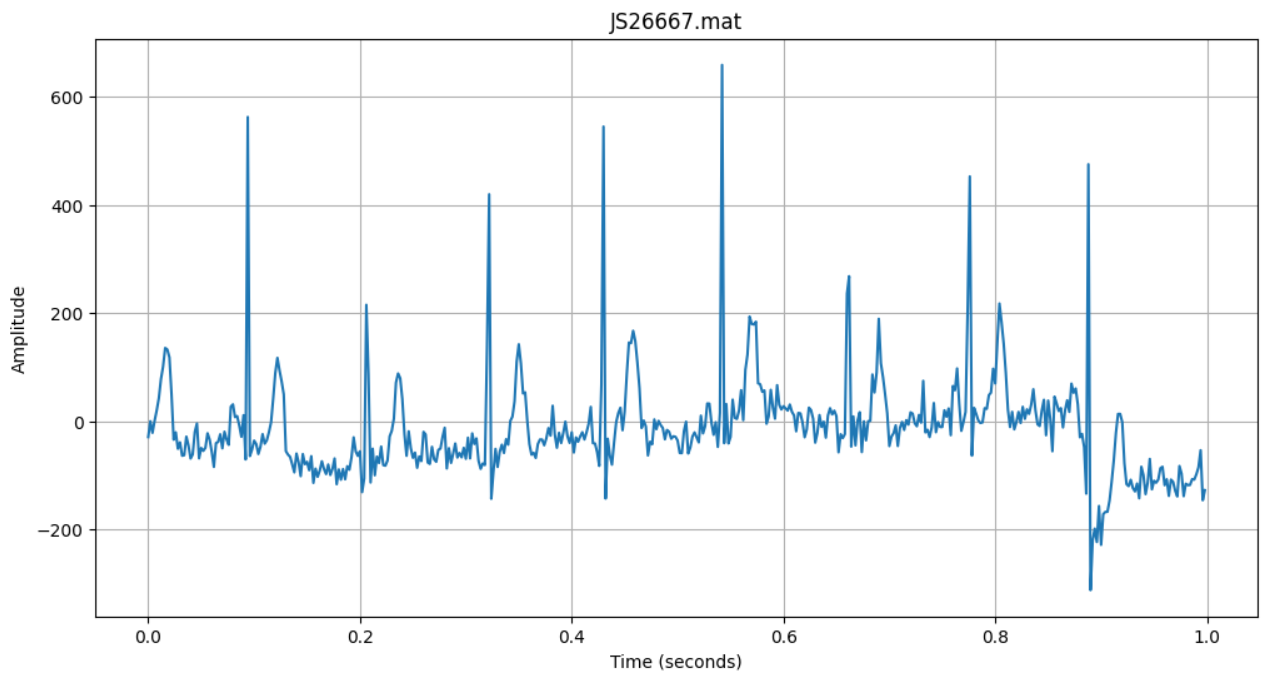
\includegraphics[width=15cm]{signal}
	\caption{Sample of a Processed ECG signal}
	\label{fig:Signal}
\end{figure}

\subsection{Important Links}\label{sec:ecg:links}
\begin{itemize}
    \item \textbf{\texttt{py-ecg-detectors} Documentation}: \href{https://pypi.org/project/py-ecg-detectors/}{https://pypi.org/project/py-ecg-detectors/}
    \item \textbf{Dataset}: \href{https://physionet.org/content/}{https://physionet.org/content/}
    \item \textbf{Guide we used for ECG Filtering}: \href{https://medium.com/@shahbaz.gondal588/understanding-ecg-signal-processing-with-python-b9dd4ea68682}{https://medium.com/@shahbaz.gondal588/understanding-ecg-signal-processing-with-python-b9dd4ea68682}
\end{itemize}


\end{document}
